\begin{center}
	\hrule
	\vspace{.4cm}
	{\textbf { \large ELEC 300 --- Electric Circuits II}}
\end{center}
{\textbf{Name:}\ David Li \hspace{\fill} \textbf{Student Number:}} \ V00818631  \\
{\textbf{Due Date:} Monday, 22 January 2018, 11:30 AM \hspace{\fill} \textbf{Assignment:} Number 2 \\
	\hrule
	
%	\listoffigures
\paragraph{Problem 1}
Assume the op amp is ideal.
\begin{enumerate}[label=(\alph*)]
	\item Calculate the power delivered to the $16 k\Omega$ resistor.
	
	\item Repeat a) with the op amp removed from the circuit, i.e., the load is directly connected to
	the $48 k\Omega$ resistor.
\end{enumerate}

\begin{figure}[H]
	\centering
	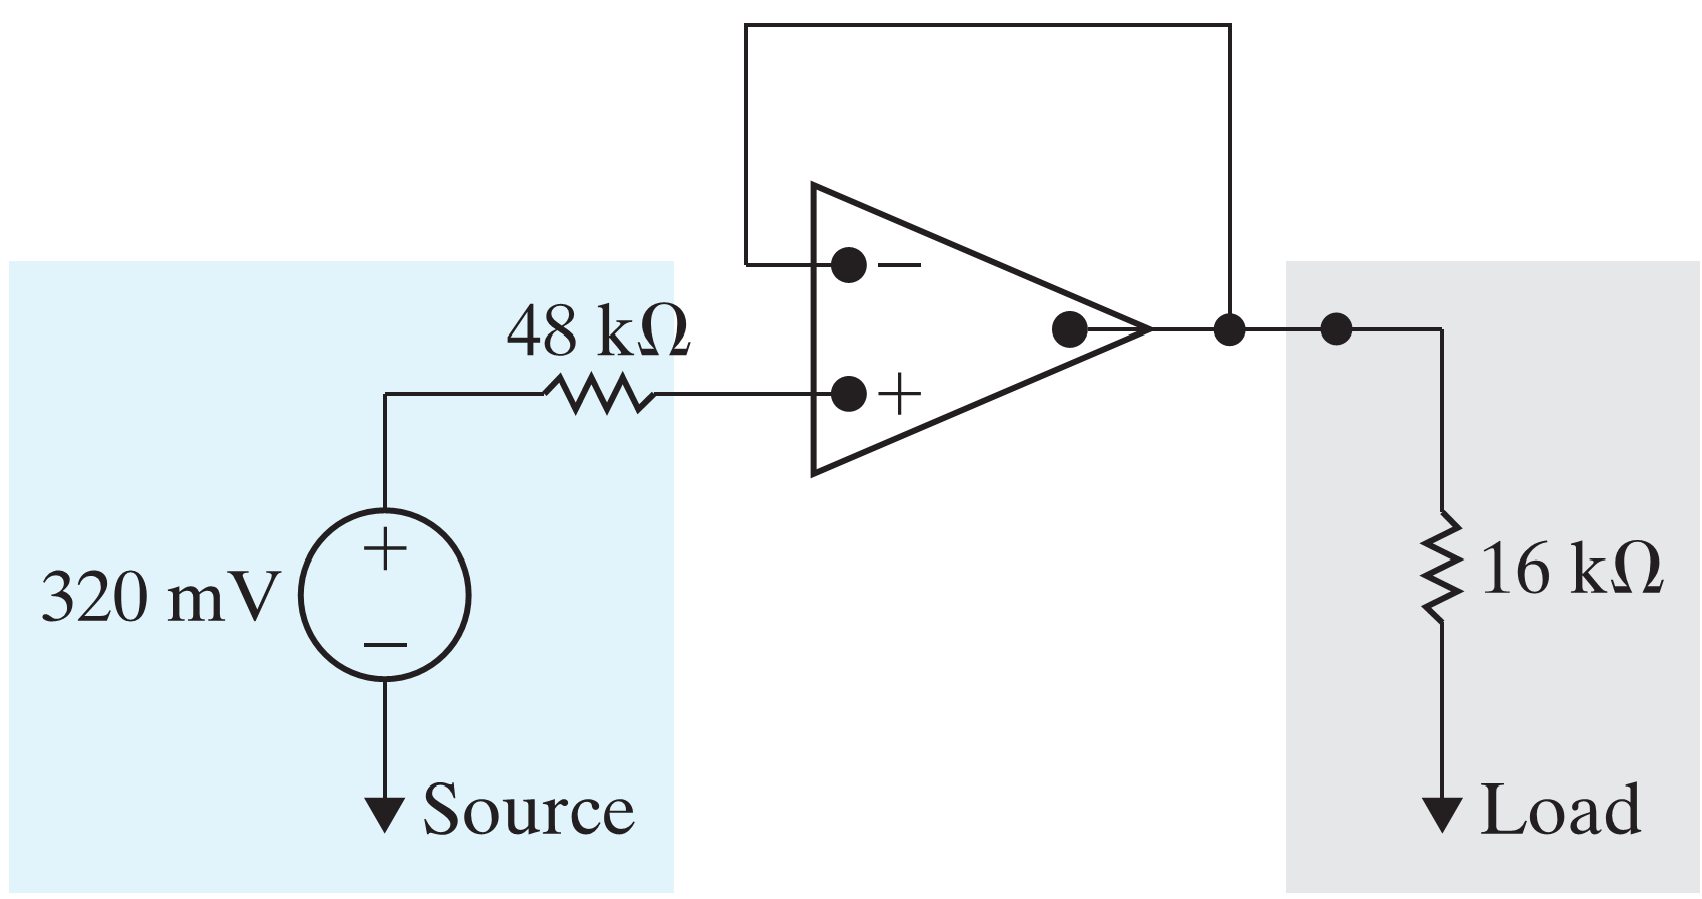
\includegraphics[width=1\linewidth]{images/P1Nillson10thQ540}
	\caption{Nillson 10th edition Q 5---40}
	\label{fig:p1nillson10thq54}
\end{figure}
In an ideal op amp, the voltage between the positive and negative terminal is the same. Since no voltage is at the ground point, all the voltage must be dropped across the $16 k \Omega$ resistor. Therefore, since $P=I^2R=V^2/R= (320 \times 10 ^{-3} V)^2 / 16 \times 10^3 \Omega = 6.4 \mu W$.

For part b) the answer is found using voltage division $v_{16 k \Omega} =\frac{16}{64}(320)=80 m V$, $p_{16 k \Omega}=\frac{(80 \times 10^{-3})^2}{16 \times 10^3}= 0.4 \mu W$

%Ignore above paragraph
\paragraph{Problem 2}

\begin{enumerate}[label=(\alph*)]
	\item Find $v_0$ if $v_a = 1V$, $v_b =1.5V$, and if $v_c = -4V$
	
	\begin{align*}
	& \frac{v_o}{220} + \frac{v_a}{44}+\frac{v_b}{27.5} + \frac{v_c}{80}=0\\
	& v_o = -6 V
	\end{align*}
	\item The voltages $v_a$ and $v_c$ remain at $1V$ and $-4V$, respectively. What are the limits on $v_b$ for the
	op amp to operate in its linear region?
	
	\begin{align*}
	& v_o -6 V - 220/27.5 v_b = \pm 10 V \\
	& v_b = \frac{(10+6)V \times 27.5}{220}= 2V, \quad v_b = \frac{-(10-6)}{8}=-0.5 V \\
	-0.5V \leq v_b \leq 2V
	\end{align*}
\end{enumerate}
\begin{figure}[H]
	\centering
	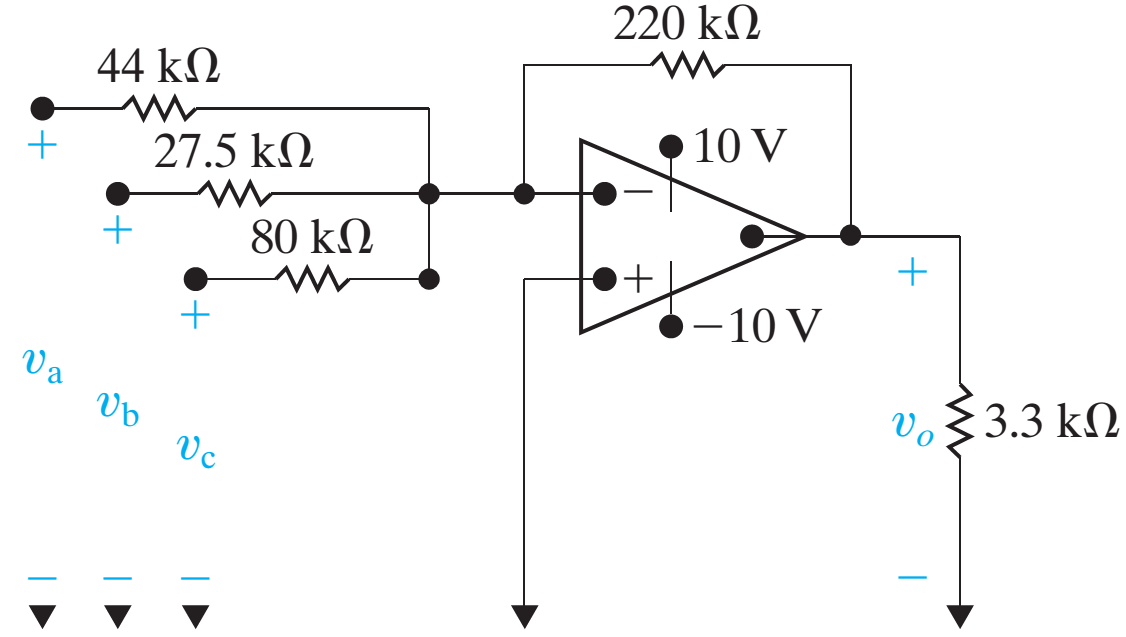
\includegraphics[width=1\linewidth]{images/P2Nillson10thQ5_12_513}
	\caption{Nillson 10th Edition Q 5-12 or 5-13}
	\label{fig:p2nillson10thq512513}
\end{figure}
\paragraph{Problem 3}
Select the values of $R_b$ and $R_f$ such that $v_o = 8000 \Omega(i_b- i_a)$.
\begin{figure}[H]
	\centering
	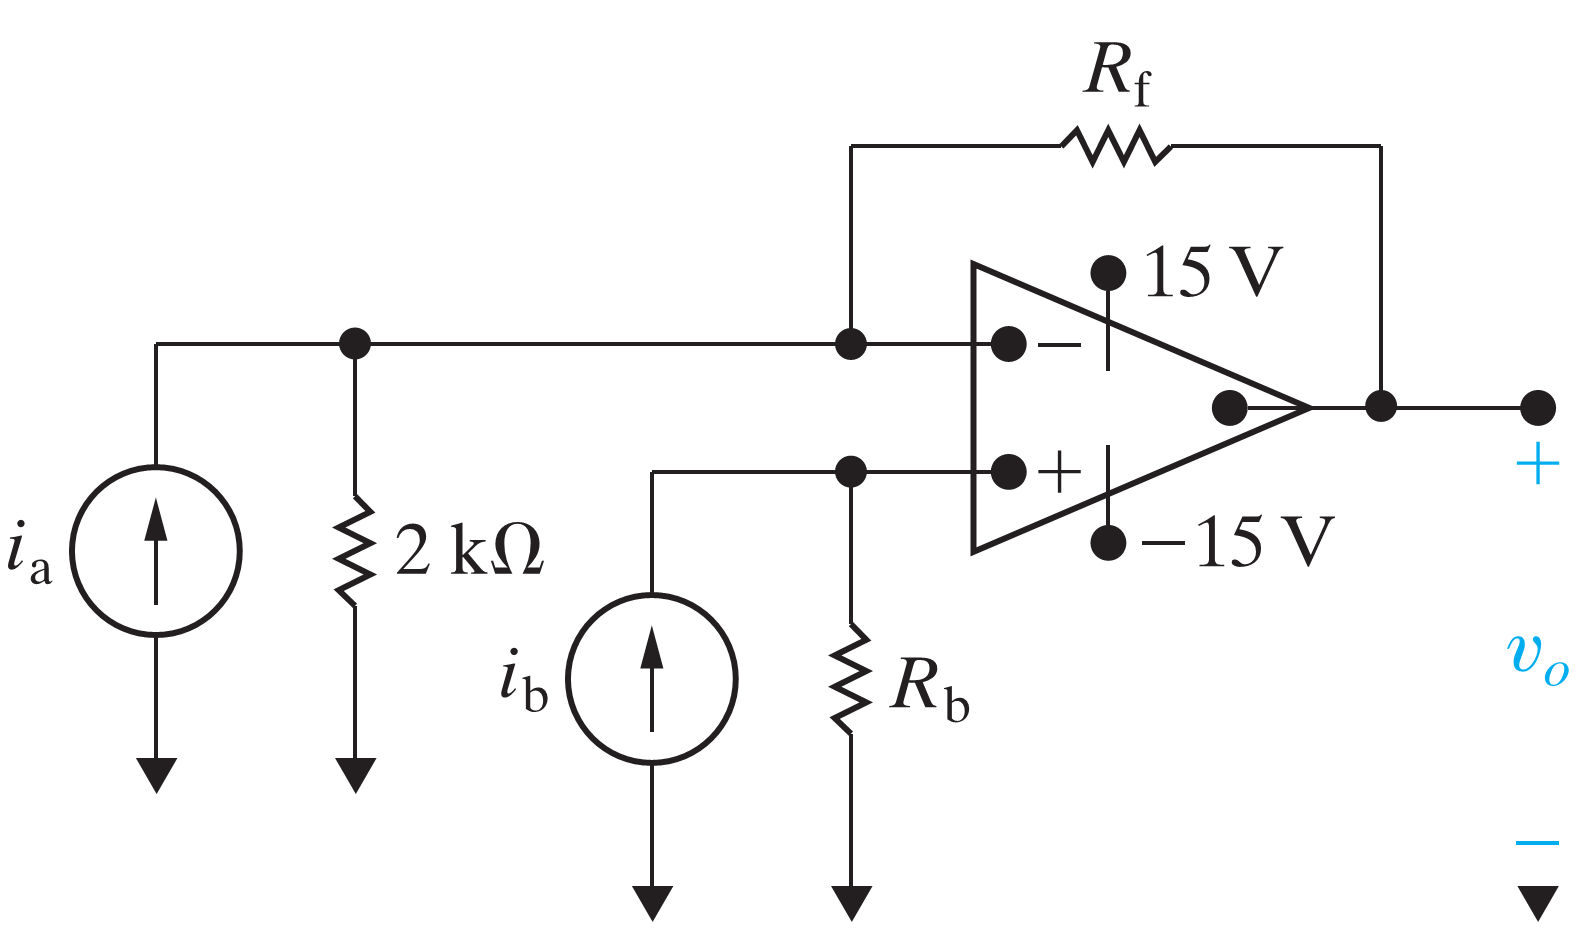
\includegraphics[width=1\linewidth]{images/P3Nillson10thQ5_31}
	\caption{Nillson 10th Edition Q 5---31}
	\label{fig:p3nillson10thq531}
\end{figure}
\begin{align*}
& v_b=R_bi_b=v_a \quad  \frac{R_bi_b}{2000}+\frac{v_a-v_o}{R_f}-i_a=0 \\
& \frac{R_bi_b}{2000}+\frac{R_bi_b-v_o}{R_f}-i_a=0 \quad R_bi_b \left(\frac{1}{2000}+\frac{1}{R_f}\right)-i_a=\frac{v_o}{R_f} \\
& R_f = 8000 k \Omega \quad R_b=1.6 k \Omega 
\end{align*}
\paragraph{Problem 4}
Determine the output voltage $v_o$.

First convert the current source to voltage source $2 \times 10^{-3}\times 5\times 10^3=10V$
\begin{figure}[H]
	\centering
	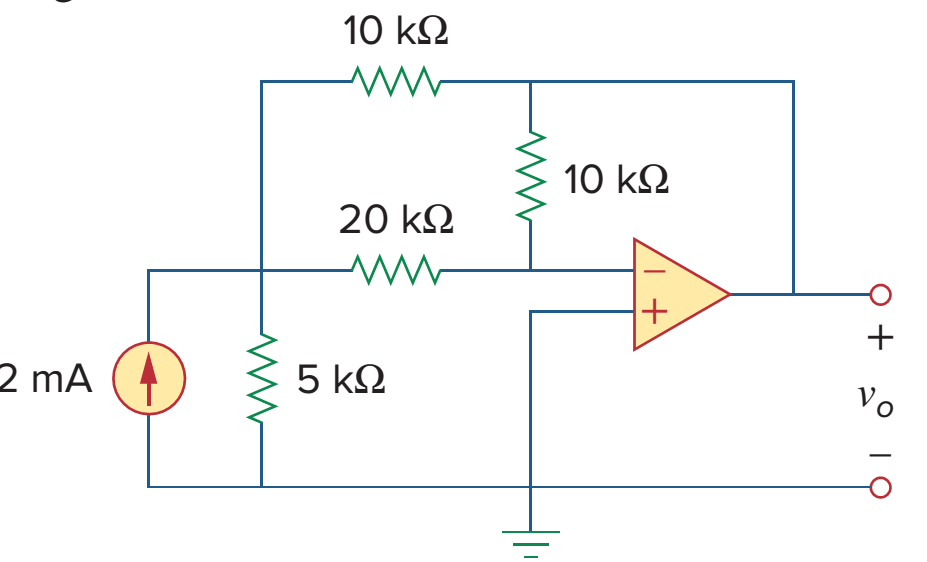
\includegraphics[width=1\linewidth]{images/P4Alexander6thQ5_14}
	\caption{Alexander 6th edition Q 5---14}
	\label{fig:p4alexander6thq514}
\end{figure}
\begin{align*}
& \frac{10-v_1}{5}=\frac{v_1-v_2}{20}+\frac{v_1-v_o}{10} \quad v_2=v_b=0\\
& \frac{10-v_1}{5}=\frac{v_1}{20}+\frac{v_1-v_o}{10} \\
& v_1=-2v_o \quad 0.35v_1 -0.1v_o=2 \quad v_o=-2.5V
\end{align*}
\paragraph{Problem 5}
Determine the voltage gain $v_o/v_i$ of the bridge amplifier
\begin{figure}[H]
	\centering
	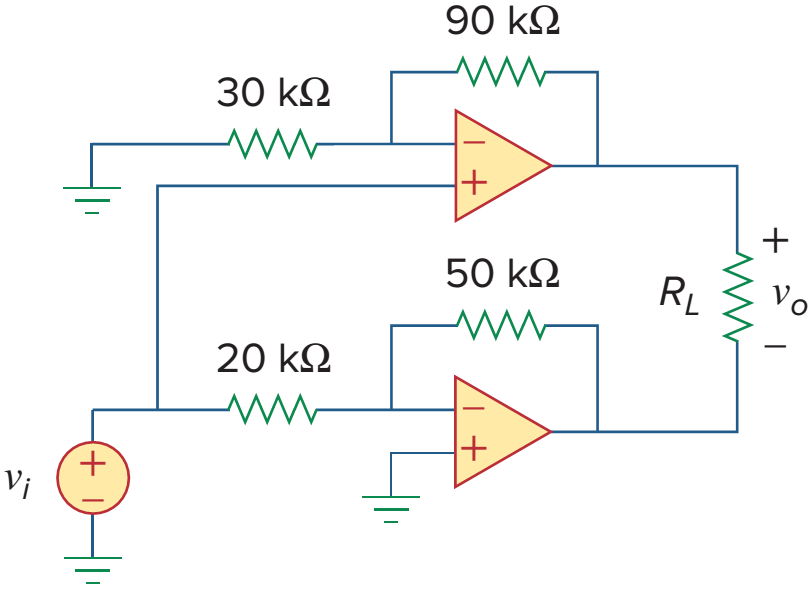
\includegraphics[width=1\linewidth]{images/P5Alexander6thQ5_92}
	\caption{Alexander 6th edition Question 5---92}
	\label{fig:p5alexander6thq592}
\end{figure}

\begin{align*}
& v_1 = (1+\frac{90}{30})v_i=4v_i\\
& v_2 = -(50 / 20)v_i=-2.5v_i \\
& v_o = v_1 -v_2 = 6.5 v_i \quad v_o / v_i = 6.5 v_i / v_i = 6.5
\end{align*}